\section{Aufbau}

\begin{minipage}{0.5\textwidth}
Maßgebend für den Aufbau ist der $50 \si{\liter}$ große, mit Edelstahl umhüllte Szintillator vom Typ \enquote{NE 102} und mit Tuluol gefüllt. Diesem ist ein eigener Abschnitt gewidmet und dort entsprechend erläutert. \ref{kommt}
Mit ihm werden die einfallenden Myonen für die Detektion sichtbar gemacht. Da die entstehenden Signale schwach sind, bietet es sich an diese durch einen Sekundärelektronenverstärker, kurz SEV zu verstärken. An diesen Verstärkern ist für
die Funnktionalität eine Hochspannung angelegt. Dieser Teil des Aufbaus ist symetrisch an beiden Stirnseiten des Szintillator angebracht. So ist es also möglich die einfallenden Teilchen als Lichtsignal durch die SEV auszulesen.
Das Signal der zwei Sekundärelektronenverstärker kann durch vielerlei Gründe einseitig verschoben sein, das heißt es tritt durch asymetrische Verzögerungen eine zeitliche Differenz $\increment t$ auf.
\end{minipage}
Die Zeitliche Differenz zwischen den SEVs kann man durch passend eingesetzte \enquote{Delays} entgegenwirken. Diese sind weiter Kabel, 
die durch ihre wählbare Länge die Zeit des Sginals verzögern. So ist es also, dass ein einfallendes Teilchen ein Signal zeitgleich an beiden Anschlüssen ankommen lässt.
Der Aufbau neigt dazu, Störeffekte durch etweige spontane Emission von Elektronen an der Photokathode, zuzulassen. Hier wird ein Diskriminator verwendet, um das Rauschcen zu filtern.
Dieses Bauteil ist direkt mit den SEVs verbunden, es gibt also zwei Individuell einstellbare Diskriminatoren. Bei diesem Elementen ist sowohl
ein \enquote{Threshhold}-, also eine Art Schwelle für die einlaufenden Impulse, und die Breite \enquote{Width} einstellbar.
Die Schwelle ermöglicht es Rauschen aus ungewollten Quellen zu Filtern, mit der Gefahr die Impulse selbst nicht mehr wahrzunehmen. 
Die Breite stellt die elektrische Impulsdauer abhängig von der Einstellung da. Gewählt wurden in dem Versuch $\SI{10}{\nano\seconds}$ und $\SI{20}{\nano\seconds}$.
Als zweite Maßnahme wird eine Koinzidenzschaltung dazugeschaltet. In diese Schaltung laufen die wahlweise mehreren Signale, hier zwei, ein und werden nur dann weitergeleited wenn dies gleichzeitig passiert.
Vorzustellen ist dieser Vorgang als logische UND Verknüpfung mit beliebig vielen Bedingungen, die ein Zeitfenster von $\increment t_k$ haben um zu wirken. 
Möglich ist es immer noch für zwei zeitgleich auftretende Emessionen von Elektronen in den SEVs ein fälschliches Signal auszulösen. Die Wahrscheinlichkeit dazu ist aber hinreichend gering
und somit zu vernachläsigen.










\begin{figure}
    \centering
    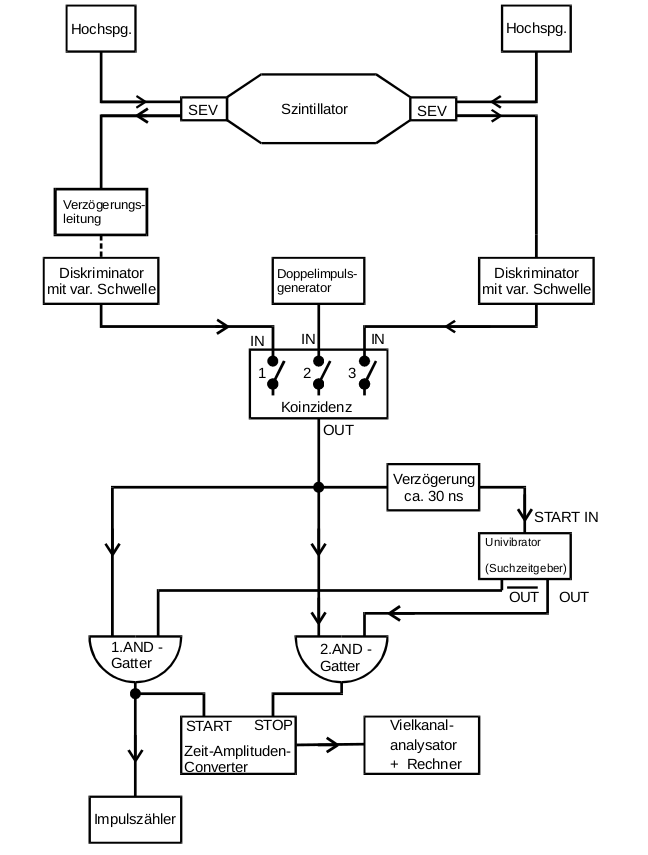
\includegraphics[width=0.6\textwidth]{bilder/aufbau.png}
    \caption{Schematischer Aufbau zur bestimmung der Lebensdauer von Myonen. \cite{skript}} 
    \label{fig:1}
\end{figure}